\documentclass[a4paper, 11pt]{article}
\usepackage{amsmath}
\usepackage{graphicx}
\usepackage{geometry}
\usepackage{listings}
\geometry{scale=0.8}
\linespread{1.5}
\usepackage{hyperref}
\usepackage{listings}


\title{	
\normalfont \normalsize
\textsc{School of Data and Computer Science, Sun Yat-sen University} \\ [25pt] %textsc small capital letters
\rule{\textwidth}{0.5pt} \\[0.4cm] % Thin top horizontal rule
\huge  E09 Variable Elimination \\ % The assignment title
\rule{\textwidth}{2pt} \\[0.5cm] % Thick bottom horizontal rule
\author{16337102 Zilin Huang}
\date{\normalsize\today}
}

\begin{document}
\maketitle
\tableofcontents
\newpage


\section{VE}

The burglary example is described as following:
\begin{figure}[h]
  \centering

  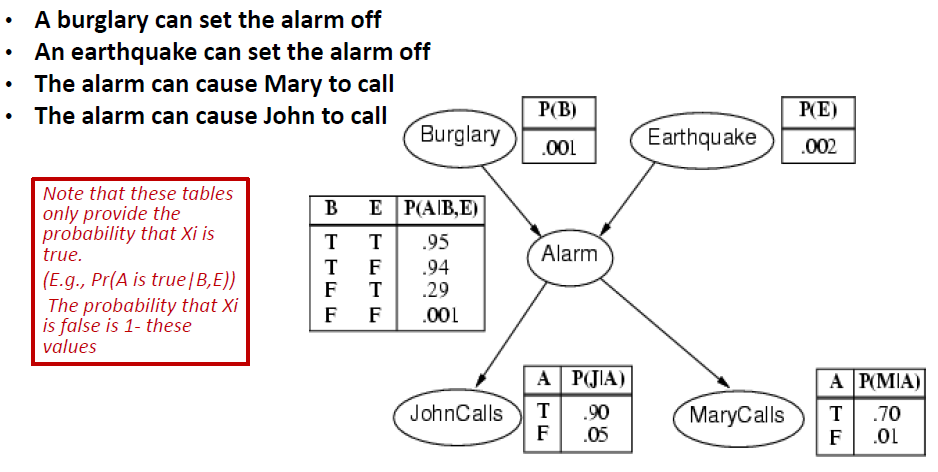
\includegraphics[width=14cm]{Pic/burglary}
\end{figure}

\begin{figure}[ht]
\centering
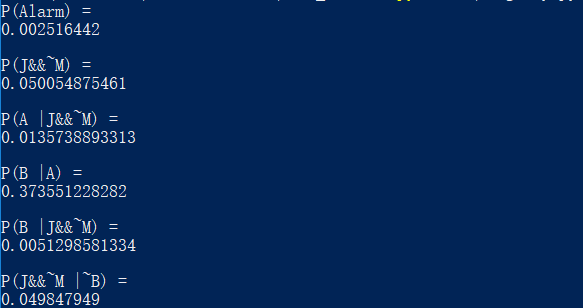
\includegraphics[width=12cm]{Pic/burglar_result}
\end{figure}
Here is a VE template for you to solve the burglary example:
\begin{lstlisting}[language=Python,frame=single]
class VariableElimination:
    @staticmethod
    def inference(factorList, queryVariables,
    orderedListOfHiddenVariables, evidenceList):
        for ev in evidenceList:
            #Your code here
        for var in orderedListOfHiddenVariables:
            #Your code here
        print "RESULT:"
        res = factorList[0]
        for factor in factorList[1:]:
            res = res.multiply(factor)
        total = sum(res.cpt.values())
        res.cpt = {k: v/total for k, v in res.cpt.items()}
        res.printInf()
    @staticmethod
    def printFactors(factorList):
        for factor in factorList:
            factor.printInf()
class Util:
    @staticmethod
    def to_binary(num, len):
        return format(num, '0' + str(len) + 'b')
class Node:
    def __init__(self, name, var_list):
        self.name = name
        self.varList = var_list
        self.cpt = {}
    def setCpt(self, cpt):
        self.cpt = cpt
    def printInf(self):
        print "Name = " + self.name
        print " vars " + str(self.varList)
        for key in self.cpt:
            print "   key: " + key + " val : " + str(self.cpt[key])
        print ""
    def multiply(self, factor):
        """function that multiplies with another factor"""
        #Your code here
        new_node = Node("f" + str(newList), newList)
        new_node.setCpt(new_cpt)
        return new_node
    def sumout(self, variable):
        """function that sums out a variable given a factor"""
        #Your code here
        new_node = Node("f" + str(new_var_list), new_var_list)
        new_node.setCpt(new_cpt)
        return new_node
    def restrict(self, variable, value):
        """function that restricts a variable to some value
        in a given factor"""
        #Your code here
        new_node = Node("f" + str(new_var_list), new_var_list)
        new_node.setCpt(new_cpt)
        return new_node
# create nodes for Bayes Net
B = Node("B", ["B"])
E = Node("E", ["E"])
A = Node("A", ["A", "B","E"])
J = Node("J", ["J", "A"])
M = Node("M", ["M", "A"])

# Generate cpt for each node
B.setCpt({'0': 0.999, '1': 0.001})
E.setCpt({'0': 0.998, '1': 0.002})
A.setCpt({'111': 0.95, '011': 0.05, '110':0.94,'010':0.06,
'101':0.29,'001':0.71,'100':0.001,'000':0.999})
J.setCpt({'11': 0.9, '01': 0.1, '10': 0.05, '00': 0.95})
M.setCpt({'11': 0.7, '01': 0.3, '10': 0.01, '00': 0.99})

print "P(A) **********************"
VariableElimination.inference([B,E,A,J,M], ['A'], ['B', 'E', 'J','M'], {})

print "P(B | J~M) **********************"
VariableElimination.inference([B,E,A,J,M], ['B'], ['E','A'], {'J':1,'M':0})
\end{lstlisting}
\section{Task}
\begin{itemize}
\item You should implement 4 functions: \texttt{inference}, \texttt{multiply}, \texttt{sumout} and \texttt{restrict}. You can turn to Figure \ref{Fig:ve_product} and Figure \ref{Fig:sumout_restrict} for help.
\item Please hand in a file named \textsf{E09\_YourNumber.pdf}, and send it to \textsf{ai\_2018@foxmail.com}
\end{itemize}


\begin{figure}[ht]{}
\centering
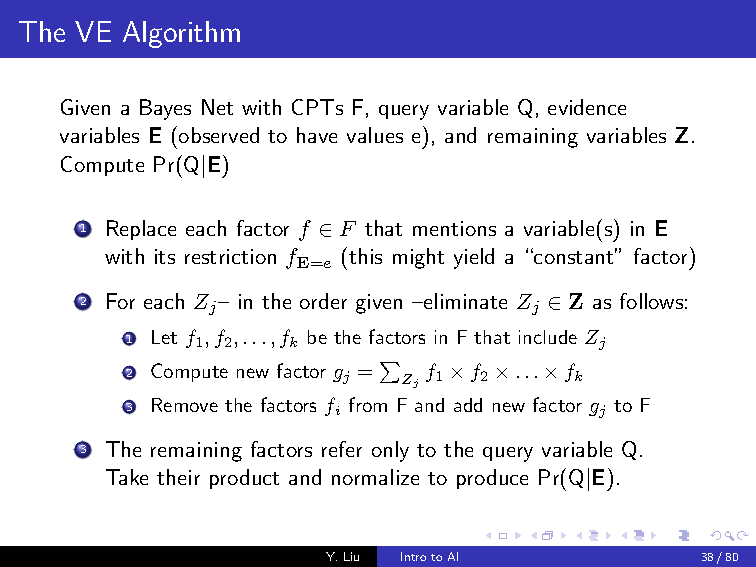
\includegraphics[width=7.5cm]{Pic/ve}
\qquad
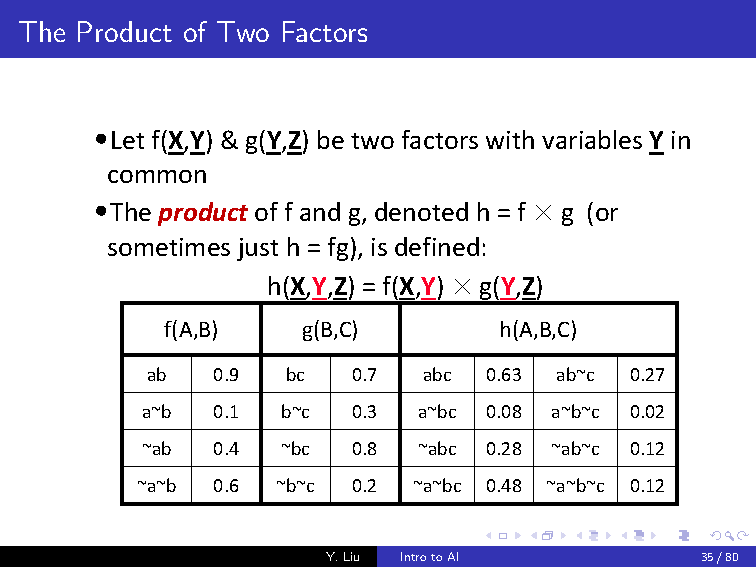
\includegraphics[width=7.5cm]{Pic/product}
\caption{VE and Product}
\label{Fig:ve_product}
\end{figure}


\begin{figure}[ht]
\centering
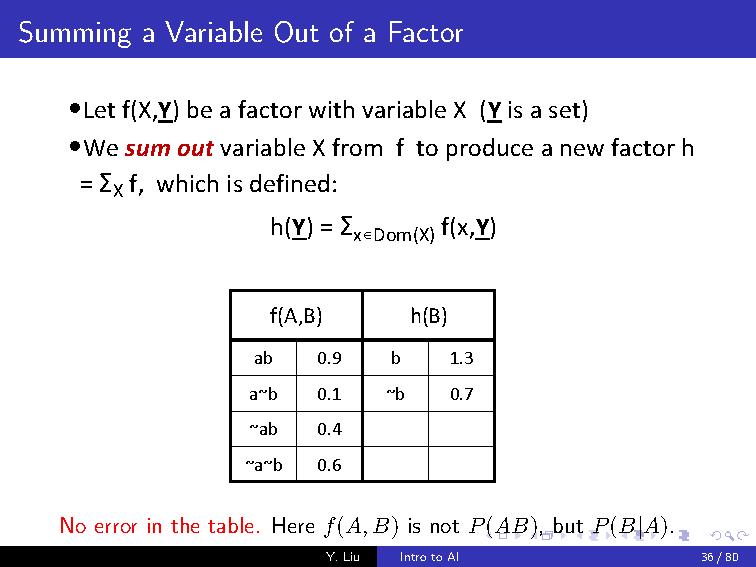
\includegraphics[width=7.5cm]{Pic/sumout}
\qquad
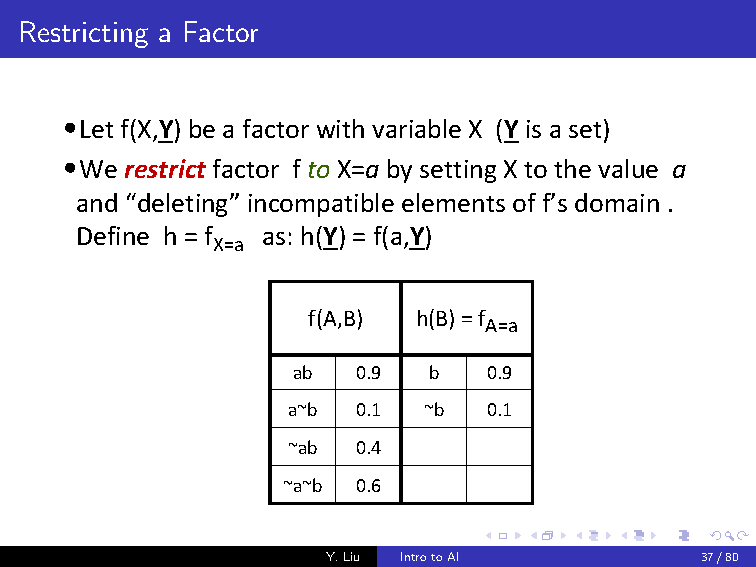
\includegraphics[width=7.5cm]{Pic/restrict}
\caption{Sumout and Restrict}
\label{Fig:sumout_restrict}
\end{figure}



\section{Codes}
\begin{lstlisting}[language=Python,frame=single]
import copy

def compare(list1, list2):
    num = len(list1)
    if num == len(list2):
        for i in range(num):
            if list1[i] != list2[i]:
                return False
        return True
    return False


def VE(factorList, queryVariables, orderedList, evidenceList):
    #restrict
    for ele, value in evidenceList.items():
        for factor in factorList:
            if ele in factor.varList:
                new_node = factor.restrict(ele, value)
                factorList.remove(factor)
                factorList.append(new_node)

    #eliminate
    for var in orderedList:
        #find factor with var
        mid_list = []
        for factor in factorList:
            if var in factor.varList:
                mid_list.append(factor)
        for factor in mid_list:
            factorList.remove(factor)

        while len(mid_list) != 1:
            for i in range(len(mid_list)):
                if i >= len(mid_list):
                    break
                ele = mid_list[i].varList[-1]
                for j in range(len(mid_list)):
                    if j >= len(mid_list):
                        break
                    if i != j:
                        ele_ = mid_list[j].varList[0]
                        if ele == ele_:
                            mid_list[i]=mid_list[i].multiply(mid_list[j])
                            del mid_list[j]

        fir = mid_list[0]
        fir = fir.sumout(var)
        factorList.append(fir)


    for factor in factorList:
        if len(factor.varList) == 0:
            factorList.remove(factor)

    tar = queryVariables[0]
    mid_list = []
    for factor in factorList:
        if tar not in factor.varList:
            mid_list.append(factor)
    for factor in mid_list:
        factorList.remove(factor)
    res = factorList[0]
    for factor in factorList[1:]:
        res = res.multiply(factor)
    #normalize
    total = sum(res.cpt.values())
    res.cpt = {k: v/total for k, v in res.cpt.items()}
    return res


class Node:
    def __init__(self, name, var_list):
        global number
        self.name = name
        self.varList = var_list
        self.cpt = {}

    def setCpt(self, cpt):
        self.cpt = cpt

    def printInf(self):
        print("Name = " + self.name)
        print(" vars " + str(self.varList))
        for key in self.cpt:
            print("   key: " + key + " val : " + str(self.cpt[key]))
        print('')

    def multiply(self, factor):  # factor is node
        new_cpt = {}
        newList = []
        if self.varList[-1] == factor.varList[0]:  # f(a, b) X g(b, c)
            # new variable list, order is important
            del factor.varList[0]
            newList = self.varList + factor.varList
            for key, value in self.cpt.items():
                for key_, value_ in factor.cpt.items():
                    new_key = list(key)
                    new_key_ = list(key_)
                    if new_key[-1] == new_key_[0]:
                        del new_key_[0]
                        result_key = new_key + new_key_  # new key
                        result_value = value * value_  # new value
                        result_key = "".join(result_key)  #list to string
                        if not new_cpt.__contains__(result_key):
                            new_cpt[result_key] = result_value
        new_node = Node("f" + str(newList), newList)
        new_node.setCpt(new_cpt)
        return new_node

    def sumout(self, variable):
        # find the position of variable
        position = self.varList.index(variable)
        new_var_list = copy.deepcopy(self.varList)
        new_var_list.remove(variable)  # delete varable
        new_cpt = {}
        for key, value in self.cpt.items():  # modify the cpt
            for key_, value_ in self.cpt.items():
                new_key = list(key)
                new_key_ = list(key_)
                if not compare(new_key, new_key_):#two keys are different
                    del new_key[position]
                    del new_key_[position]
                    if compare(new_key, new_key_):
                        new_key = "".join(new_key)
                        value = value + value_
                        if not new_cpt.__contains__(new_key):
                            new_cpt[new_key] = value
                        break
        new_node = Node("f" + str(new_var_list), new_var_list)
        new_node.setCpt(new_cpt)
        return new_node

    def restrict(self, variable, value):
        position = self.varList.index(variable)
        new_var_list = copy.deepcopy(self.varList)
        new_var_list.remove(variable)  # delete varable
        new_cpt = {}
        for key, value_ in self.cpt.items():  # modify the cpt
            new_key = list(key)
            if int(new_key[position]) == value:  # item in new cpt
                del new_key[position]
                key_ = "".join(new_key)
                new_cpt[key_] = value_  # new cpt
        new_node = Node("f" + str(new_var_list), new_var_list)
        new_node.setCpt(new_cpt)
        return new_node

def initial():
    B = Node("B", ["B"])
    E = Node("E", ["E"])
    A = Node("A", ["B", "E", "A"])
    J = Node("J", ["A", "J"])
    M = Node("M", ["A", "M"])

    B.setCpt({'1': 0.001, '0': 0.999})
    E.setCpt({'1': 0.002, '0': 0.998})
    A.setCpt({'111': 0.95, '110': 0.05, '101': 0.94, '100': 0.06,
            '011': 0.29, '010': 0.71, '001': 0.001, '000': 0.999})
    J.setCpt({'11': 0.9, '10': 0.1, '01': 0.05, '00': 0.95})
    M.setCpt({'11': 0.7, '10': 0.3, '01': 0.01, '00': 0.99})
    return [B, E, A, J, M]



print("P(A) =")
factorList = initial()
res = VE(factorList, ['A'], ['B', 'E', 'J', 'M'], {})
p_A = res.cpt["1"]
p_a = res.cpt["0"]
print(p_A)

print("P(B | J~M) =")
factorList = initial()
res = VE(factorList, ['B'], ['A', 'E'], {'J': 1, 'M': 0})
p_B_Jm = res.cpt["1"]
print(p_B_Jm)

print("P(A | J~M) =")
factorList = initial()
res = VE(factorList, ['A'], ['B', 'E'], {'J': 1, 'M': 0})
p_A_Jm = res.cpt["1"]
print(p_A_Jm)

print("P(B | A) =")
factorList = initial()
res = VE(factorList, ['B'], ['E', 'J', 'M'], {'A': 1})
p_B_A = res.cpt["1"]
print(p_B_A)


factorList = initial()
res = VE(factorList, ['J'], ['B', 'E', 'A'], {'M': 0})
p_J_m = res.cpt["1"]

factorList = initial()
res = VE(factorList, ['M'], ['B', 'E', 'J'], {'A':1})
p_M_A = res.cpt["1"]
p_m_A = res.cpt["0"]

factorList = initial()
res = VE(factorList, ['M'], ['B', 'E', 'J'], {'A': 0})
p_M_a = res.cpt["1"]
p_m_a = res.cpt["0"]

p_m = p_m_A * p_A + p_m_a * p_a
p_Jm = p_m * p_J_m
print("P(J&&~M) =")
print(p_Jm)

p_B = 0.001
p_b = 1 - p_B
p_b_Jm = 1 - p_B_Jm
p_Jm_b = p_b_Jm * p_Jm / p_b
print('P(~B|J&&~B) =')
print(p_Jm_b)
\end{lstlisting}

\section{Results}
\begin{figure}[h]
  \centering

  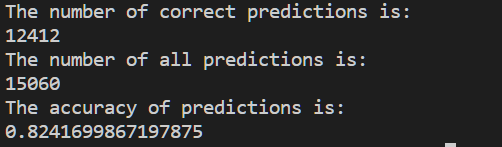
\includegraphics[width=14cm]{result.png}
\end{figure}

%\clearpage
%\bibliography{E:/Papers/LiuLab}
%\bibliographystyle{apalike}
\end{document}
%%% Local Variables:
%%% mode: latex
%%% TeX-master: t
%%% End:
